\documentclass[12pt,a4paper]{article} 
\usepackage[portuguese]{babel} \usepackage[utf8]{inputenc}
\usepackage{amsmath} 
\usepackage{graphicx}
\usepackage{booktabs}
\usepackage{float}
\begin{document}
\setcounter{figure}{4}
\setcounter{section}{3}
\setcounter{page}{5}
\section{Relatório}
\subsection{Introdução}

Nesta prática, deseja-se entender o funcionamento de um circuito integrado temporizador \emph{LM555}, e suas aplicações como um multivibrador monoestável e como um multivibrador astável (cirucito oscilador). 

Um vibrador monoestável é um circuito eletrônico que gera um pulso de saída. Quando desencadeado, um pulso de duração pré-defnida é produzido.
O circuito então retorna para seu estado de repouso e não produz outro sinal de saída até ser desencadeado novamente.

Um multivibrador é um circuito eletrônico usado para implementar uma variedade de dispositivos simples de dois estados como osciladores de relaxação, timers e flip-flops.
Ele consiste de dois dispositivos amplificadores (transistores, tubos de vácuo ou outros dispositivos) acoplado com resistores e capacitores.
O primeiro circuito multivibrador, o circuito multivibrador astável, foi inventado por Henri Abraham e Eugene Bloch durante a primeira guerra mundial. 
Eles chamaram de circuito multivibrador pois a forma de onda da saída era rica em harmônicos. 
Já um multivibrador astável é um circuito que não está estável em nenhum estado; continuamente troca de um estado para outro. Este funciona como oscilador de relaxação.




\subsection{Análises}
No experimento 1, escolhemos os valores de resistência e capacitância adequado a fim de obter um pulso de duração previamente escolhida, no caso $1ms$. Este valor foi escolhido através do datasheet e verificado através da montagem do circuito.   O resultado
se encontra na Figura~\ref{fig:1}
\begin{figure}[htpb]
  \centering
  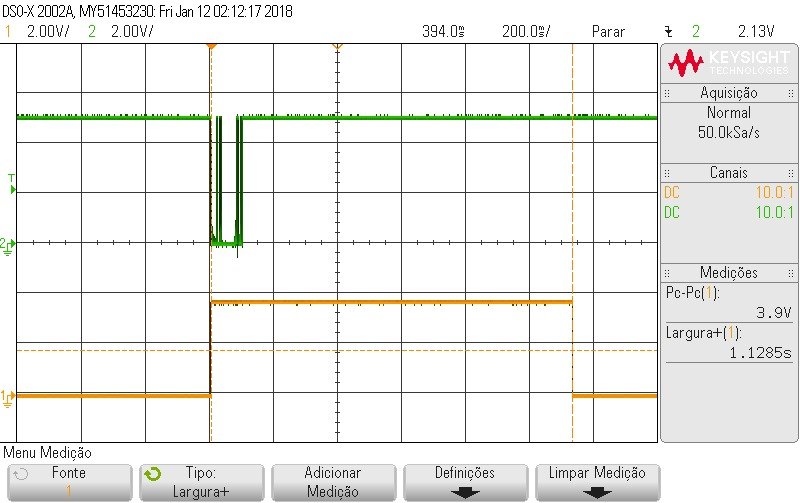
\includegraphics[width=0.8\linewidth]{img/exp1.jpg}
  \caption{Name}
  \label{fig:1}
\end{figure}

No experimento 2, 
\subsection{Conclusão}
\end{document}
